\documentclass[10pt]{article}
%\documentclass[review]{siamart1116}
%\documentclass[review]{siamonline1116}

\usepackage{amsmath}
\usepackage{amsfonts}
\usepackage{amssymb}
\usepackage{fancyhdr}
\usepackage[margin=0.75in]{geometry}
\usepackage{graphicx}
\usepackage[section]{placeins}
\usepackage{nicefrac}
\usepackage{bm}
\usepackage{xcolor}
\usepackage[format=plain,indention=.5cm, font={it,small},labelfont=bf]{caption}
\usepackage{subcaption}
\usepackage{float}
\usepackage{enumerate}
\usepackage{tikz}
\usetikzlibrary{arrows.meta}
\usepackage[all]{xy}
\usepackage{url}
\usepackage{multicol}



%%%%%%%%%%%%%%%%%%%%%%%%%%%%%%%%%%%%%%%%%%%%%%%%%%%%%%%%%%%%%%%%%%%%%%%%%%%%%%%%%%%%%%%%%%%%%%%%%%%%%%%%%%%%%%%%%%
\usepackage{stackengine}
\usepackage{amsthm}
\usepackage{cleveref}


\newtheorem{theorem}{Theorem}
\newtheorem*{theorem*}{Theorem}
\newtheorem{lemma}{Lemma}
\newtheorem*{lemma*}{Lemma}
\newtheorem{conj}{Conjecture}
\newtheorem{corollary}{Corollary}
\newtheorem{clm}{Claim}
\newtheorem{rmk}{Remark}
\newtheorem{note}{NOTE}
\newtheorem{method}{Method}
\newtheorem*{method*}{Method}

\theoremstyle{definition}
\newtheorem*{def*}{Definition}
\newtheorem{definition}{Definition}
\numberwithin{theorem}{section}
\numberwithin{definition}{section}
\numberwithin{lemma}{section}
\numberwithin{corollary}{section}
\numberwithin{clm}{section}
\numberwithin{rmk}{section}

\newcommand{\low}[1]{$_{\text{#1}}$}
\newcommand\xput[2][0.5]{%
	\rule{#1\linewidth}{0pt}\makebox[0pt][c]{#2}\hfill}

\setlength{\headheight}{15pt}
\pagestyle{fancy}
\renewcommand{\headrulewidth}{0pt}
\fancyhead[L]{Brunner}
\fancyhead[C]{Co-Occurrance Network}
\fancyhead[R]{\today}
\lfoot{}
\cfoot{\thepage}
\rfoot{}

%%%%%%%%%%%%%%%%%%%%%%%%%%%%%%%%%%%%%%%%%%%%%%%%%%%%%%%%%%%%%%%%%%%%%%%%%%%%%%%%%%%%%%%%%%%%%%%%%%%%%%%%%%%%%%%%%%
%
%
%\newsiamthm{clm}{Claim}
%\newsiamremark{rmk}{Remark}
%\newsiamremark{note}{NOTE}
%\numberwithin{theorem}{section}
%
%
%%%%%%%%%%%%%%%%%%%%%%%%%%%%%%%%%%%%%%%%%%%%%%%%%%%%%%%%%%%%%%%%%%%%%%%%%%%%%%%%%%%%%%%%%%%%%%%%%%%%%%%%%%%%%%%%%%
\newenvironment{inbox}[1]
{\begin{center}
		\begin{tabular}{|p{0.9\textwidth}|}
			\hline
			{\bf #1}\\
		}
		{ 
			\\\\\hline
		\end{tabular} 
	\end{center}
}
\newenvironment{inbox2}
{\begin{center}
		\begin{tabular}{|p{0.9\textwidth}|}
			\hline \vspace{-0.5 cm}
		}
		{ 
			\\ \hline
		\end{tabular} 
	\end{center}
}




\newcommand{\nhalf}{\nicefrac{1}{2}}
\newcommand{\eps}{\epsilon_{machine}}
\newcommand{\ol}{\overline}
\renewcommand{\b}{\bm}

\definecolor{dgreen}{RGB}{49,128,23}
\definecolor{lgreen}{RGB}{77, 255, 166}
\definecolor{nicepink}{RGB}{255, 0, 102}
\definecolor{nicered}{RGB}{255, 80, 80}
\definecolor{lblue}{RGB}{102, 163, 255}
\definecolor{lgray}{RGB}{217, 217, 217}

\newcommand{\bE}{\mathbb{E}}
\newcommand{\bP}{\mathbb{P}}
\newcommand{\bR}{\mathbb{R}}
\newcommand{\bN}{\mathbb{N}}
\newcommand{\bZ}{\mathbb{Z}}
\newcommand{\bQ}{\mathbb{Q}}
\newcommand{\bC}{\mathbb{C}}
\newcommand{\cA}{\mathcal{A}}
\newcommand{\cB}{\mathcal{B}}
\newcommand{\cC}{\mathcal{C}}
\newcommand{\cD}{\mathcal{D}}
\newcommand{\cE}{\mathcal{E}}
\newcommand{\cF}{\mathcal{F}}
\newcommand{\cG}{\mathcal{G}}
\newcommand{\cH}{\mathcal{H}}
\newcommand{\cI}{\mathcal{I}}
\newcommand{\cJ}{\mathcal{J}}
\newcommand{\cK}{\mathcal{K}}
\newcommand{\cL}{\mathcal{L}}
\newcommand{\cM}{\mathcal{M}}
\newcommand{\cN}{\mathcal{N}}
\newcommand{\cO}{\mathcal{O}}
\newcommand{\cP}{\mathcal{P}}
\newcommand{\cQ}{\mathcal{Q}}
\newcommand{\cR}{\mathcal{R}}
\newcommand{\cS}{\mathcal{S}}
\newcommand{\cT}{\mathcal{T}}
\newcommand{\cU}{\mathcal{U}}
\newcommand{\cV}{\mathcal{V}}
\newcommand{\cW}{\mathcal{W}}
\newcommand{\cX}{\mathcal{X}}
\newcommand{\cY}{\mathcal{Y}}
\newcommand{\cZ}{\mathcal{Z}}

\newcommand{\inter}{\text{\normalfont int}}
\newcommand{\ka}{\kappa}
\newcommand{\fp}{\varrho}
\newcommand{\problem}[2]{ \ \\ {\bf #1} {\it #2} \ \\} 

\renewcommand{\arraystretch}{1.5}
\renewcommand{\thefootnote}{\fnsymbol{footnote}}	
\author{Jim Brunner}
\title{Correlation and Co-occurrence Networks in Taxonomic Classification}

\begin{document}
\maketitle

\section{Introduction}
\cite{edge}\cite{gottcha}\cite{ecol_net_rev}\cite{mic_int}\cite{machine_learning}\cite{PhysRevE.70.056131}\cite{PhysRevE.70.066111}\cite{cyotscape}\cite{gut}
\section{Network Construction}

\subsection{Correlation construction}
We construct an undirected, weighted graph with nodes from the set of taxa in the GOTTCHA output of metagenomic samples. Edges correspond to correlation between taxa across samples. If $\b{x}$ is the vector of abundances of a certain taxa, and $\b{y}$ is the vector of abundances of another, we compute the correlation of these two vectors (with $N$ samples):
\[
\rho_{xy} = \frac{1}{N}\frac{(\b{x}- \mu_x\b{1}) \cdot (\b{y} - \mu_y\b{1})}{\sigma_x \sigma_y}
\]
where $\mu_x$ is the mean abundance of taxa $x$, and $\sigma_x$ is the standard deviation of abundance of taxa $x$ across samples. These correlations can be efficiently computed from a matrix whose columns correspond to the GOTTCHA output (in taxa abundance) of metagenomic samples, and rows corresponding to the abundances of taxa across samples. Finally, if $\b{r}_i$ is the vector of abundances of taxa $i$, and $\b{r}_k$ is a vector of abundances of taxa $k$, we compute
\[
w_{ik} = \left\{\begin{array}{c c}
\rho_{\b{r}_i\b{r}_k} & \rho_{\b{r}_i\b{r}_k}\geq 0.8\\
0 &  \rho_{\b{r}_i\b{r}_k}< 0.8
\end{array}\right.
\]
and take an edge from taxa $i$ to taxa $k$ with weight $w_{ik}$ (where an edge with weight $0$ implies no edge).

Alternatively, we can first ``thresh-hold" the abundances given, converting to binary presence/absence data. To do this, we find the mean of all non-zero abundance values $\mu_{nz}$, and take
\[
r^*_{ij} = \left\{\begin{array}{c c}
1 & r_{ij} \geq 0.01\mu_{nz}\\
0 & r_{ij} < 0.01 \mu_{nz}
\end{array}\right.
\]
where $r_{ij}$ is the the abundance of taxa $i$ in sample $j$. The network is then constructed using correlation just as before.

Again, we check the significance of each edge, removing edges that have a high probability of occurring in a null model. We check this using Monte-Carlo simulation by estimating $p_{ik} \approx P(\rho_{\b{r}_i^{null}\b{r}_k^{null}} > \rho_{\b{r}_i\b{r}_k})$. In construction, we take enough Monte-Carlo trials for a $95\%$ confidence interval of length $0.03$. We then adjust edges so that
\[
p_{ik} > 0.05 \Rightarrow w_{ik} = 0
\]

\subsection{Null Model}\label{null}
Rather than simply generate an Erd\H{o}s-R\'{e}nyi random graph with some chosen parameter, we generate a graph that more closely reflects the idea of random data. That is, we start with random data that resembles our real data, and then generate a graph. The random data is generated in the following way. Let 
\[
N_j = |\{i: r_{ij} \neq 0\}|
\]
and 
\[
P_i = \frac{|\{j: r_{ij}\neq 0 \}|}{|\{(i,j): r_{ij}\neq 0 \}|}
\]
then take 
\[
\hat{r}_{ij} = \mathit{binom}(N_j,P_i)
\]
as randomly generated abundance data. The values $N_i$ are the counts of appearances of taxi $i$, while the values $P_j$ are the proportions of all appearances which happen within each sample. 
		
Then, we construct our null model graph from this random data. If $\hat{\b{r}}_i$ is the vector of random ``abundances" of taxa $i$, the null graph has edges
\[
w_{ik}^{null} = \frac{1}{N}\frac{(\b{\hat{\b{r}}_i}- \hat{\mu}_i\b{1}) \cdot (\hat{\b{r}}_k - \hat{\mu}_k\b{1})}{\hat{\sigma}_i \hat{\sigma}_k}
\]

The null model's use of a binomial random variable can be interpreted in the following way. A ``success" for a taxa/sample pair is an appearance of the taxa in the sample. The number of trials is the number of times the taxa appears in the data set. The probability of success is the proportion of all appearances which happen within the sample. This does have some drawbacks: notably that it does not preserve total abundance, or even total appearances. It allows more than one ``success" for a single taxa/sample pair, which could be interpreted as higher abundance. Our ``random samples" should be scaled by average abundances of a taxa across samples to ``look like" real data. This doesn't effect correlation, because $\mathit{Cov}(ax,by) = ab\mathit{Cov}(x,y)$, and $\sigma_x = \mathit{Cov}(x,x)^{\nhalf}$, implying that $w_{ik} = \mathit{Cor}(\hat{\b{r}}_i,\hat{\b{r}}_k) =  \mathit{Cor}(a\hat{\b{r}}_i,b\hat{\b{r}}_k)$. 

In \cite{coocc}, this model is called the ``binomial model". Interestingly, that paper argues that an ``edge swapping" model is more accurate, but slower to construct and so less suitable for Monte-Carlo methods. A random permutation of the data used in \cite{gut}.

\subsection{Significance of the network}\label{sig}
The networks connected by the methods above would not occur in randomized data, and so there is some significance to these networks. In a Monte-Carlo simulation, networks are generated according to the null mode in order to estimate the following
\begin{itemize}
	\item $P(\mu_d < \mu_d^{null})$, where $\mu_d$ is the mean degree of the nodes of a network
	\item $P(\sigma_d < \sigma_d^{null})$, where $\sigma_d$ is the variance of degrees of the nodes of a network
	\item $P(\lambda_{max} < \lambda_{max}^{null})$, where $\lambda_{max}$ is the largest eigenvalue of the adjacency matrix
	\item $P(\lambda_{min} < \lambda_{min}^{null})$, where $\lambda_{min}$ is the smallest eigenvalue of the adjacency matrix
	\item $P(|\cE| < |\cE^{null}|)$
\end{itemize} 

The result with $10,000$ Monte Carlo trials show that it was extremely rare for a network constructed from the null model to have higher mean degree, higher degree variance, larger maximum eigenvalue, smaller minimum eigenvalue, or more edges. This suggests that the networks constructed from real data would be very unexpected according to the null model. 
\begin{figure}
	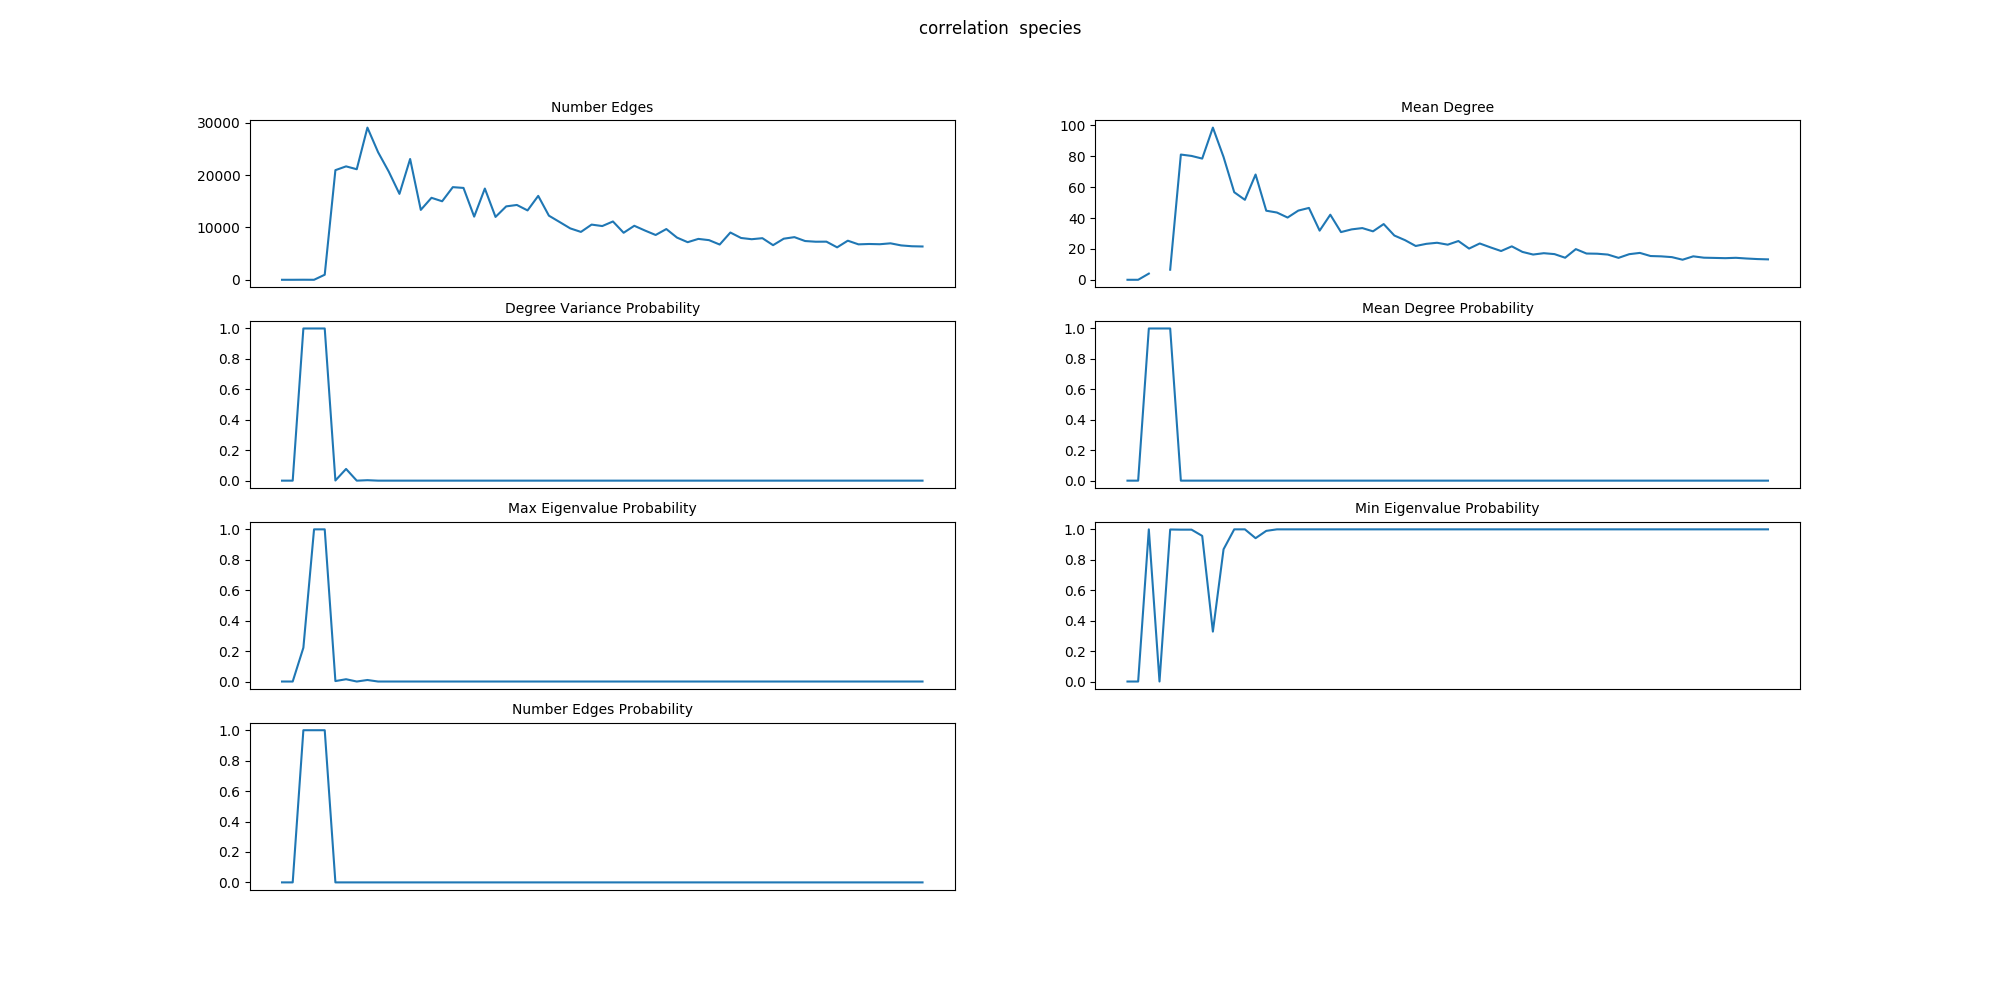
\includegraphics[scale = 0.4]{../../stat_figs/pears_1000__species.png}
	\caption{The result of Monte-Carlo estimation of the likelihood of various network statistics, as well as the number of edges and mean degree. The networks were made from correlations using randomly drawn subsets of increasing size of the data at the species level, from 1 sample to 60 samples. Samples were GOTTCHA output of data from (FIND OUT). For each network, 1000 random trials were generated according to the above null model in order to estimate likelihood of statistics.}\label{montecarlos}
\end{figure}



\section{Taxonomic Classification Analysis}


We would like to identify taxa likely to be present in a sample, given an initial estimate of abundances of taxa. Inspired by spectral clustering, we may solve the diffusion equation on the graph in order to identify nodes that are likely present, given the sample data. The diffusion equation is
\[
\frac{\partial}{\partial t} u(v,t) = L u(v,t)
\]
where $v$ takes values in the vertex set of the graph. Then, we encode ``known" information in the initial values.

\begin{inbox2}
	\begin{method}[Initial Value Problem]\label{initalCond}
		Let $u_i(t)$ be the solution at node $v_i$ to the discrete diffusion problem
		\[
		\frac{d}{dt}\b{u}(t)  = - L\b{u}
		\]
		where $L$ is the  graph Laplacian with initial conditions $u_i = 1$ if node $v_i$ is known to be ``on", $u_j = 0$ if $v_j$ is known to be ``off", and $u_k = 0.5$ (or $0$, or perhaps encoded with some confidence in $[0,1)$) if $v_k$ is unknown. I then normalize the initial vector so that it represents a probability distribution on the nodes.
		
		Then, if $\b{K}$ is the information ``known" and the values of $v_{k}$ and $v_{l}$ are unknown,
		\[
		\int_0^{\infty} u_k(t) dt - \int_0^{\infty} u_l(t) dt >  0 \Rightarrow  P(v_k=  1|\b{K}) > P(v_l = 1|\b{K})
		\]
	\end{method}
\end{inbox2}
These comparisons are easily computed. Solutions to the diffusion equation are of the form
\[
\b{u} = \sum_{i=1}^a c_i \b{1}|_{cc} + \sum_{i=a+1}^n c_i e^{-\lambda_i t} \b{\xi}_i 
\]
where $a$ is the number of connected components of the graph, and $\lambda_i,\b{\xi}_i$ are eigenvalue, eigenvector pairs of $L$. Note that each eigenvalue $\lambda_i \geq 0$, with $\lambda_i>0$ for $i = a+1,...,n$ \cite{vonLuxburg2007}. Then, assuming there is some initial mass on the connected component containing $v_1$ and $v_2$, 
\[
\int_0^{\infty} u_k(t) dt - \int_0^{\infty} u_l(t) dt =   \sum_{i=a+1}^n c_i  (\xi_{ki} - \xi_{li}) \int_0^{\infty} e^{-\lambda_i t} dt = \sum_{i=a+1}^n \frac{c_i}{\lambda_i}  (\xi_{li} - \xi_{ki}) 
\]
and $\b{c} = V^{-1}\b{u}(0)$. Therefore, it is straightforward to compute and compare the transitive terms of the solution:
\begin{equation}\label{ivp_computation}
\int_0^{\infty}\left( u_k(t) - \sum_{i=1}^a c_i \right) dt = \sum_{i=a+1}^n \frac{c_i}{\lambda_i}\xi_{ki}
\end{equation}


We can relate this method to spectral clustering. Spectral clustering using computes a $k$-means clustering algorithm on the rows for a matrix of the first $k$ eigenvectors $\xi_k$. Thus, spectral clustering uses a distance metric from the inner product
\[
\|u_l\|_s = \b{(V^T)_l}^T \begin{pmatrix}
\b{I}_{k\times } & 0 \\
0 & \b{0}_{n-k \times n-k} 
\end{pmatrix}
\b{(V^T)_l}
\]
and clusters nodes $l$ and $m$ if $\|u_l- u_m\|_s$ is small, or
\begin{equation}
\langle u_m, u_l\rangle_{sc} = (\b{V}^T_m)^T \begin{pmatrix}
\b{I}_{k\times } & 0 \\
0 & \b{0}_{n-k \times n-k} 
\end{pmatrix}
\b{V}^T_l
\end{equation}
is large. Similarly, inspection of \cref{ivp_computation} reveals that we will rank nodes highly when
\begin{equation}
\langle \b{V}^{-1} \b{u}(0) , u_l\rangle_{ivp}  = (\b{V}^{-1}\b{u}(0))^T\b{\Lambda}^{-1} \b{V}^T_l
\end{equation}
is large.  Notice that the ordering of the eigenvalues insures that the terms on the diagonal of $\b{\Lambda}^{-1}$ decay along the diagonal, and all terms are positive, making this matrix and the matrix used in \cref{ivp_computation} similar. We are in some sense then asking about how close a node is to the initial condition given in a metric similar to that used in spectral clustering. In fact, if we have as an initial condition $\b{u}(0) = \b{V} \b{V}_m^T$, this metric is very close to that used in spectral clustering.

This method provides a ranking of taxa which attempts to estimate an ordering of the probabilities 
\[
\bP(t_i \in S | m(S))
\]
where $t_i \in S$ indicates taxa $i$ is present in a sample, and $m(S)$ is the GOTTCHA output for the sample.

\subsection{Matching samples to networks}

Suppose we have different networks built from different types of data - i.e. healthy and unhealthy, or different regions, etc. We would like to match a sample with the network that makes most the sense. That is, we would like to say that a sample is more likely to be from one type of data than the other based on the network.

If the sample ``fits" a network well, \cref{initalCond} should return nodes ranked highly which have nonzero and perhaps high abundance. If we imagine a sample is created by performing a random walk on a graph and recording the nodes most often visited, \cref{initalCond} should identify nodes that the random walk ``should" have seen often. If there are a bunch of those missing from the sample, we might think the network is not the right one. We could consider the map from rank to abundance, and integrate this against a kernel that weights towards the high ranks. Let $\b{s}$ be the sample abundances (so $s_i$ is the abundance of organism $i$), and $\b{\sigma}$ the ranking. We take 
\[
F(\b{s},\b{\sigma}) =\frac{1}{\|\b{s}\|} \sum_{i=1}^n c^{\nicefrac{\sigma_i}{n}} s_i
\]
where $c<1$. Given a sample, we get ranking from a network $N_j$. Let $\b{\sigma}^j(\b{s})$ be the ranking given by diffusion on network $j$. Then,
\[
F_j(\b{s}) = F(\b{s},\b{\sigma}^j(\b{s})) = \frac{1}{\|\b{s}\|} \sum_{i=1}^n c^{\nicefrac{\sigma^j_i}{n}} s_i
\]
and we can attempt to optimize over the networks. We can then conjecture
\begin{conj}
	Assume that $F_j(\b{s}) > F_k(\b{s})$. Then $P(\b{s}|N_j) > P(\b{s}|N_k)$.
\end{conj}

We begin with a very simple example. Consider the two networks shown in \cref{more_tests}. Using ``samples" $u_1 = (\nicefrac{1}{6},\nhalf,\nicefrac{1}{3},0,0,0)$, $u_2 = (\nicefrac{1}{6},\nhalf,0,0,\nicefrac{1}{3},0)$, and $u_3= (0,0,0,\nicefrac{1}{6},\nhalf,\nicefrac{1}{3})$ gave results shown in \cref{tiny_res}.


\begin{figure}
	\begin{subfigure}[b]{0.46\linewidth}
		\begin{center}
			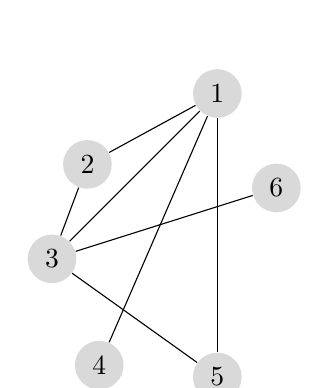
\begin{tikzpicture}[scale = 1.5]
			\node (a) at (1,2.3) [circle, fill = lgray] {$1$};
			\node (d) at (0,0) [circle, fill = lgray] {$4$};
			\node (c) at (-0.4,0.9) [circle, fill = lgray] {$3$};
			\node (b) at (-0.1,1.7) [circle, fill = lgray] {$2$};
			\node (e) at (1,-0.1) [circle, fill = lgray] {$5$};
			\node (f) at (1.5,1.5) [circle, fill = lgray] {$6$};
			\draw (a) edge (b);
			\draw (a) edge (c);
			\draw (b) edge (c);
			\draw (a) edge (d);
			\draw (a) edge (e);
			\draw (c) edge (f);
			\draw (c) edge (e);
			\end{tikzpicture}
		\end{center}
		\caption{Network $A_1$}
	\end{subfigure}
	\begin{subfigure}[b]{0.46\linewidth}
		\begin{center}
			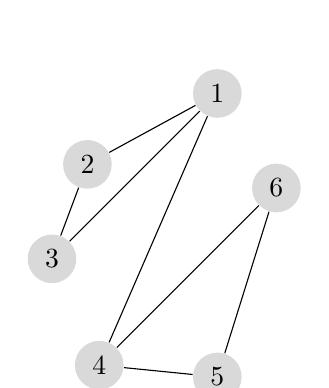
\begin{tikzpicture}[scale = 1.5]
			\node (a) at (1,2.3) [circle, fill = lgray] {$1$};
			\node (d) at (0,0) [circle, fill = lgray] {$4$};
			\node (c) at (-0.4,0.9) [circle, fill = lgray] {$3$};
			\node (b) at (-0.1,1.7) [circle, fill = lgray] {$2$};
			\node (e) at (1,-0.1) [circle, fill = lgray] {$5$};
			\node (f) at (1.5,1.5) [circle, fill = lgray] {$6$};
			\draw (a) edge (b);
			\draw (a) edge (c);
			\draw (b) edge (c);
			\draw (a) edge (d);
			\draw (e) edge (d);
			\draw (d) edge (f);
			\draw (f) edge (e);
			\end{tikzpicture}
		\end{center}
		\caption{Network $A_2$}
	\end{subfigure}
	\caption{Test networks. }\label{more_tests}
\end{figure}

\begin{figure}
	\begin{center}
		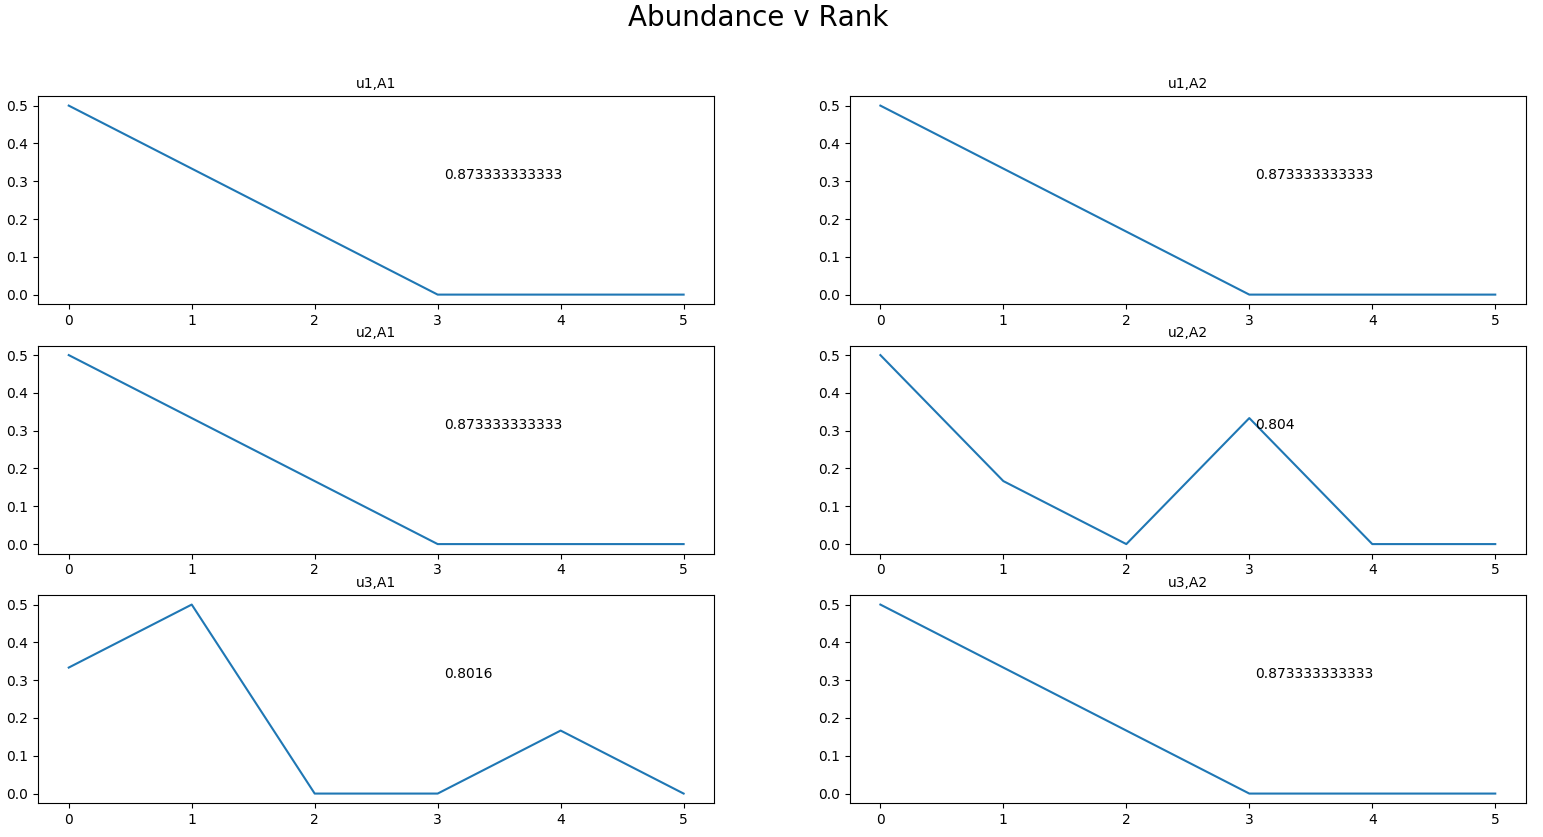
\includegraphics[scale = 0.4]{../tiny.png}	
	\end{center}
	\caption{Results of sample assignment: $u_1$ cannot be decided, $u_2$ is assigned to network $A_1$, and $u_3$ is assigned to network $A_2$.}\label{tiny_res}
\end{figure}

We performed the same experiment on a column of training data for the species level network, a column of data that was held out of the network building, and a randomly generated sample. The results, shown in \cref{full_assign}, have the training data and held out data more likely to ``fit" the network than the random data.

\begin{figure}
	\begin{subfigure}[b]{0.9\linewidth}
		\begin{center}
			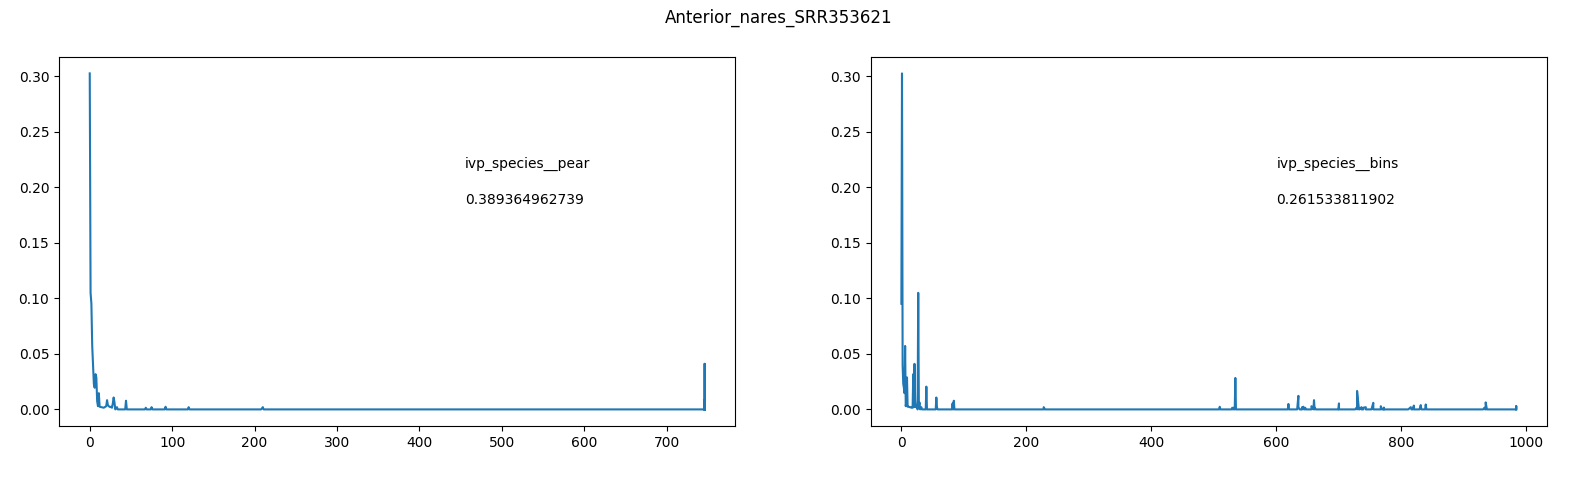
\includegraphics[scale = 0.45]{../a_nares.png}	
		\end{center}
		\caption{Assignment of column of training data to networks built with binning (right) and with correlation (left).}
	\end{subfigure}
	\begin{subfigure}[b]{0.9\linewidth}
		\begin{center}
			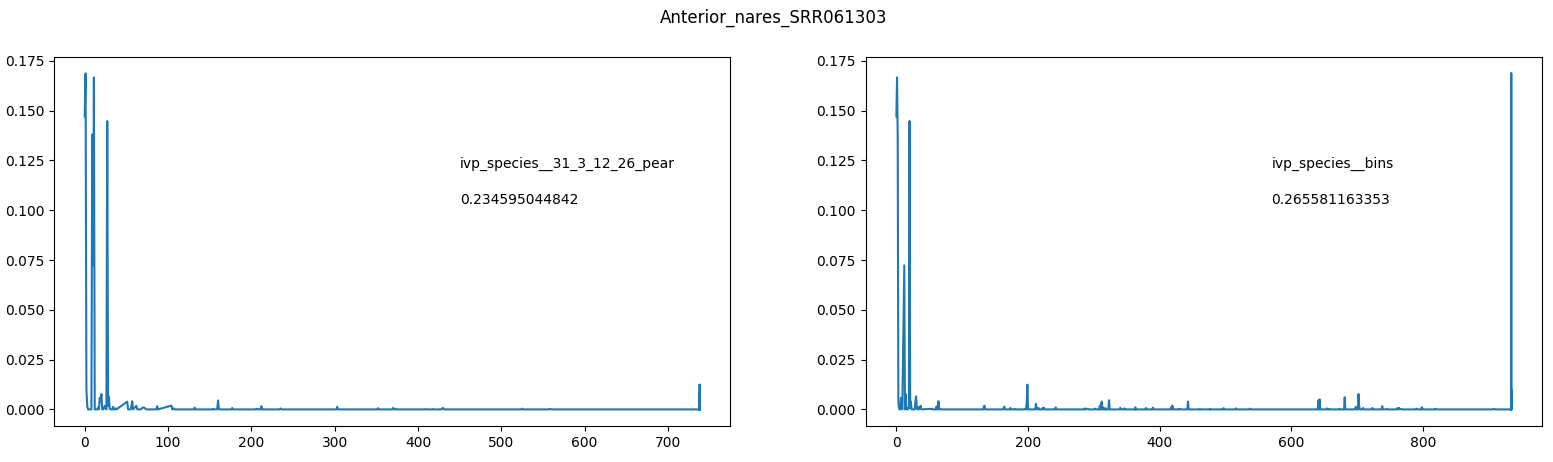
\includegraphics[scale = 0.45]{../hldouts.png}	
		\end{center}
		\caption{Assignment of column of held out data to networks built with binning (right) and with correlation (left).}
	\end{subfigure}
	\begin{subfigure}[b]{0.9\linewidth}
		\begin{center}
			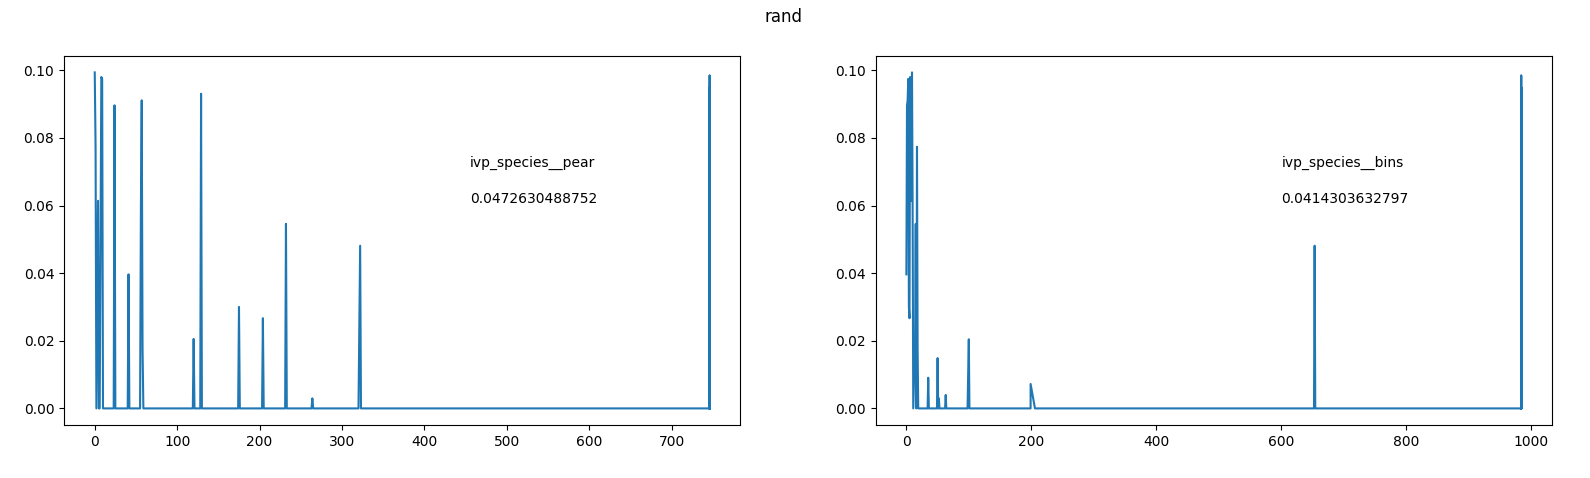
\includegraphics[scale = 0.45]{../random.png}	
		\end{center}
		\caption{Assignment randomly generated data to networks built with binning (right) and with correlation (left). This random sample had 63 nodes chosen to be present, uniformly, and given an abundance drawn from a $unif[0,0.1]$ distribution.}
	\end{subfigure}
	\caption{A training data column fits the network better than a randomly generated sample.}\label{full_assign}
\end{figure}

\section{Validation}

To validate this approach, we built correlation and thresholded correlation networks from GOTTCHA output of 1,367 samples from the NIH Human Microbiome Project (\verb|08_14_14_57_networks|). We constructed a network using all of these samples, as well as networks for 6 body sites for which at least 50 samples were present in the full 1,367:
\begin{itemize}
	\item Anterior Nares (168 samples) 
	\item Buccal Mucosa (206 samples)
	\item Posterior Fornix (110 samples)
	\item Stool (288 samples)
	\item Supragingival Plaque (220 samples)
	\item Tongue Dorsum (223 samples)
\end{itemize}
For each network we assessed the significance of the statistics listed in \cref{sig}. (\verb|stats.txt| in the folder with the networks.)

We analyzed 300 samples from the NIH Human Microbiome Project that were not used in the network training. We computed the fit score of each sample on a the networks made from the set of 1,367 samples, as well as the body site networks. We hoped to analyze the fit score's use in identifying the body site a sample was taken from. We compared fit of each sample across networks to identify the body site. 

\begin{figure}
	\begin{center}
	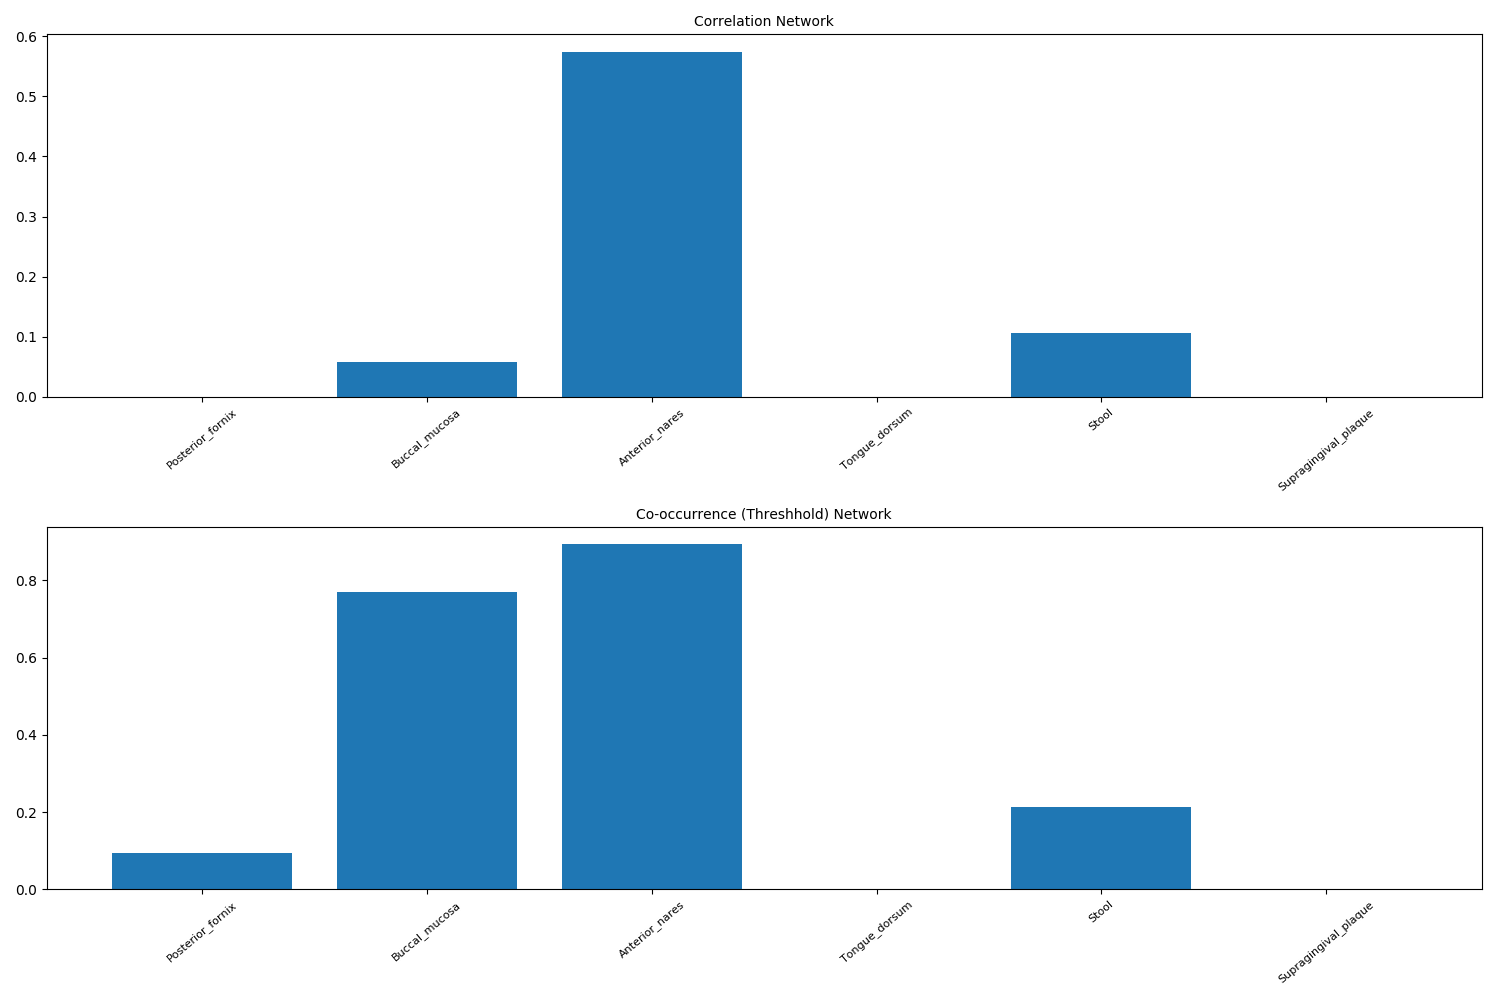
\includegraphics[scale = 0.4]{../correct_ids.png}
	\end{center}
	\caption{Proportion of samples from each body site that were correctly assigned to their body site by taking the best fit to the various body site networks (genus level).}
\end{figure}

We also computed the fit on the full networks of simulated samples created using the null model describe in \cref{null}.

\begin{figure}
	\begin{center}
	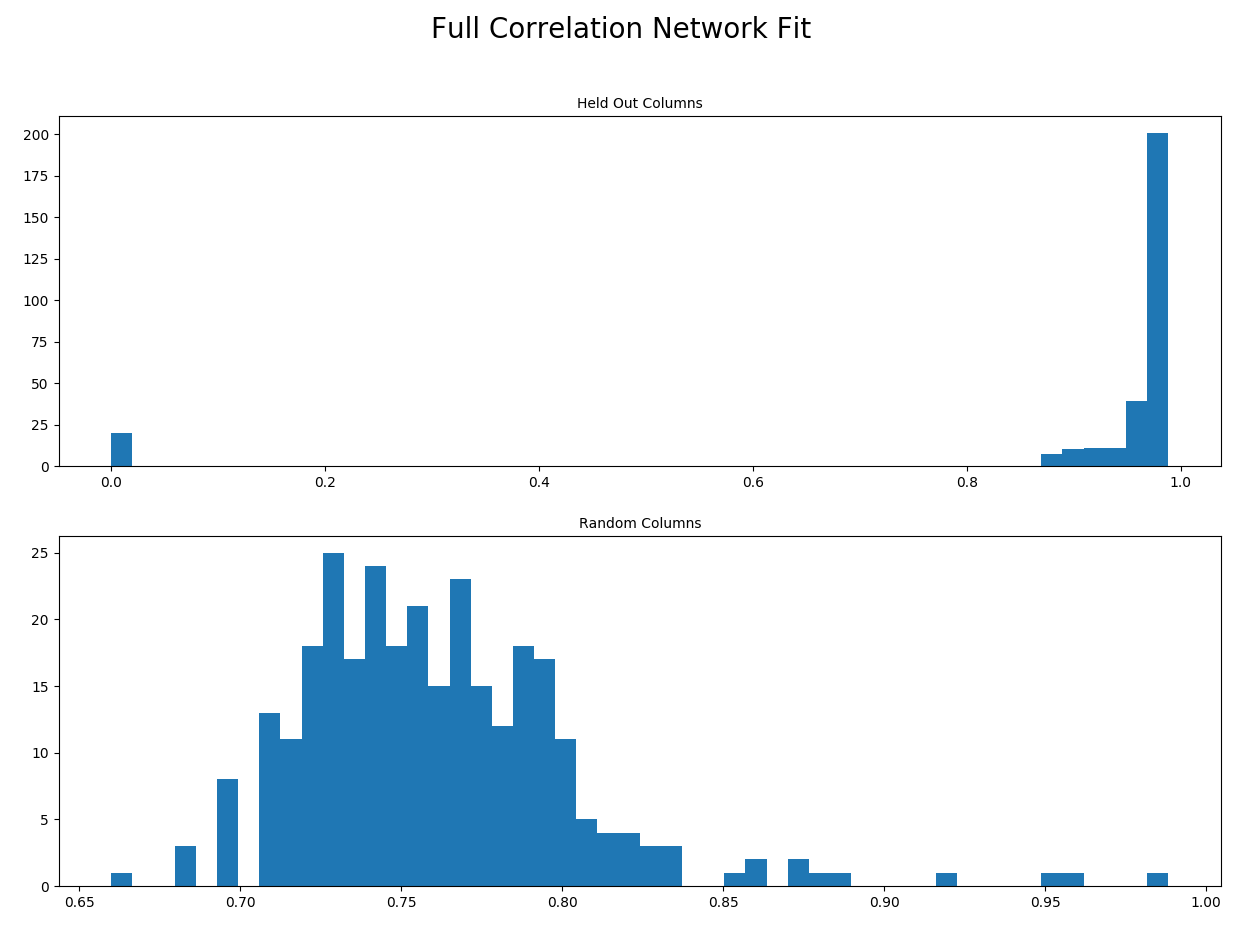
\includegraphics[scale = 0.4]{../fit_histo_cor.png}
	\end{center}
	\caption{Network fit scores of 300 hold out columns (top) to the correlation network built with all of the data, and fit of 300 simulated samples (bottom) constructed using the null model described in \cref{null} (genus level).}
\end{figure} 

For each sample, we also performed the following experiment. We set the taxa with $n^{th}$ highest abundance in the sample to $0$ abundance and used the diffusion method to find the rank of this taxa, for $n$ from 1 to 100.

\begin{figure}
	\begin{subfigure}[h]{0.45\textwidth}
		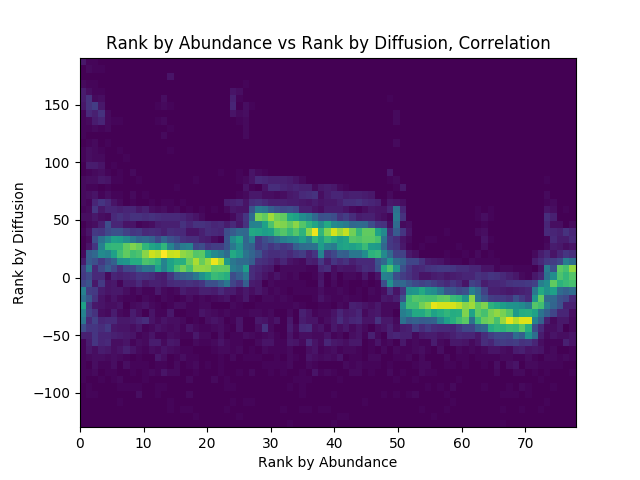
\includegraphics[scale = 0.5]{../rank_v_rank_cor.png}
		\caption{Result with correlation network. (This is weird and looks like a bug, but it may be an artifact of the fact that there aren't enough non-zero entries in the columns at the genus level. That doesn't explain the weird periodicity though)}
	\end{subfigure}
	\begin{subfigure}[h]{0.45\textwidth}
	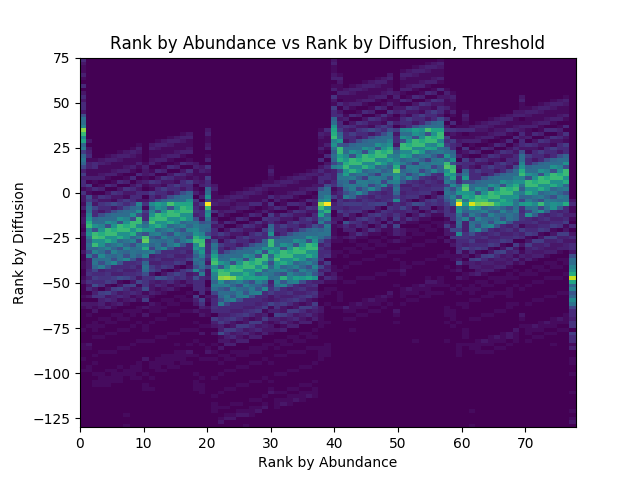
\includegraphics[scale = 0.5]{../rank_v_rank_thr.png}
	\caption{Result with thresholded correlation network. (This is weird and looks like a bug, but it may be an artifact of the fact that there aren't enough non-zero entries in the columns at the genus level. That doesn't explain the weird periodicity though)}
\end{subfigure}
\caption{Results of set the taxa with $n^{th}$ highest abundance in the sample to $0$ abundance and used the diffusion method to find the rank of this taxa, for $n$ from 1 to 100. The plots are histograms of the result, and the ``diffusion rank" plotted is the node rank minus the number of non-zero values in the sample. Thus, a rank less than zero indicates the taxa is ranked higher (after being ``removed" from the sample) than some taxa with non-zero abundance (genus level).}
\end{figure}

\section{Discussion}

\bibliographystyle{plain}
\bibliography{../summer17}
\end{document}